\documentclass[10pt,twoside,slovak,a4paper]{article}

\usepackage[slovak]{babel}
\usepackage[T1]{fontenc}
\usepackage[utf8]{inputenc}
\usepackage{graphicx}
\usepackage{booktabs}
\usepackage{url} % príkaz \url na formátovanie URL
\usepackage{hyperref} % odkazy v texte budú aktívne (pri niektorých triedach dokumentov spôsobuje posun textu)

\usepackage{cite}
\usepackage{natbib}
\usepackage{times}
\usepackage[dvips,dvipdfm,a4paper,centering,textwidth=14cm,top=4.6cm,headsep=.6cm,footnotesep=1cm,footskip=0.6cm,bottom=3.8cm]{geometry}

\pagestyle{headings}

\title{Nanoboty v medicíne}

\author{Jaroslav Sumbal, Andrej Švec\\[2pt]
	{\small Slovenská technická univerzita v Bratislave}\\
	{\small Fakulta informatiky a informačných technológií}\\
	{\small \texttt{sumbal13@fiit.stuba.sk, svec13@fiit.stuba.sk}}\\
	{\small Hlavný zdroj: \cite{Zdroj}}
	}

\date{\small 21. február 2015} % upravte



\begin{document}

\maketitle


\begin{abstract}
Rakovina je zákerná choroba a dodnes sú mnohé jej formy nevyliečiteľné. Pozrime sa na to, ako by sa tento problém dal riešiť pomocou umelej inteligencie a pokročilej technológie.

\end{abstract}

\section{Problémové prostredie}

Problémové prostredie je ľuďské telo. Je totiž veľmi zraniteľné. Stačí malý pád a zlomenina je na svete. Našťastie, väčšinu týchto fyzických zranení vieme napraviť, alebo si telo pomôže samo. Toto neplatí pre prípad zákernej choroby, akou je rakovina. Čo je to rakovina? Rakovina vznikne vtedy, keď sa niektoré bunky začnú chorobne množiť a brániť zdravým bunkám vykonávať svoju prácu. V dnešnej dobe existuje viacero druhov liečenia rakoviny, ale nefungujú dokonale. Nedajú sa vyliečiť všetky druhy rakoviny a niekedy sa dá len spomaliť ich priebeh. Preto je potrebné nové riešenie, ktoré ponúka pole nanotechnológii.

Ľuďské telo je veľmi komplikované a preto treba veľmi inteligetné riešenie. Je potrebné rozoznať zdravé bunky od tých chorých, aby sa pacientovi náhodou neprihoršilo. Ďalšia nevyhnutnosť je dobrý transportný systém. Telo už taký má, je to krvný obeh. Avšak krvný obeh ponúka plejádu možností, veľa rôznych ciest. Ktorou sa vydať? Táto otázka potrebuje premyslenú odpoveď, aby bola liečba čo najefektívnejšia.

Veľký problém taktiež predstavuje imunitný systém ľuďského tela. Ako presvedčiť telo, že nanoboty sú preň dobré, aby ich nezničilo? Nie je to vôbec ľahké, keď si uvedomíme, že niekedy je aj transplantovaný orgán odvrhnutý, teda niečo prirodzené telu. A tu je treba aby prijalo niečo syntetické. Je to jeden zo základných problémov, ktorý treba vyriešiť, aby vôbec celý tento výskum mal zmysel.

\section{Opis znalostného konateľa}

\subsection{Ciele}
Nanoboty sú vpustené do organizmu za účelom ozdravenia organizmu a to odstránením rakovinotvorných buniek prítomných v organizme. Takisto je cieľom, aby bolo minimalizované množstvo zdravých buniek, ktoré boli zničené pri odstraňovaní rakovinotvorných buniek. Teda je dôležité aby pri odstraňovaní chorých buniek neboli poškodené a zničené aj zdravé bunky. Nakoniec ide aj o minimalizáciu času potrebného na nájdenie rakovinotvornej bunky od doby jej vzniku.

\subsection{Vnemy}
Vstupmi pre nanobota sú rôzne chemické látky, ktoré nájde v bunkách a ich koncentrácia, tvar bunky, sekvencia DNA, ktorú vie prečítať. Keďže nanobot musí vedieť komunikovať s ostatnými nanobotmi, tak je pre neho vstupom aj ľubovoľná informácia od ostatných nanobotov ako aj od serveru, s ktorým nanoboti komunikujú a ktorý je mimo organizmu. Ide najmä o informácie o sekvenciách DNA a o koncentrácii rôznych chemických látok v krvi a v bunkách.

\subsection{Akcie}
Nanobot musí na základe vnemov vedieť reagovať, a to buď zničením, alebo ponechaním bunky. Najdôležitejším faktorom je pri tomto procese, správne rozlíšenie zdravej bunky od chorej bunky. Pri tomto je nutné použiť rôzne analýzy, ďalej opísané v časti \ref{sec:spravanie}. Pri týchto analýzach je nutné, aby nanobot vedel komunikovať ostatným nanobotom a serveru informácie.


\section{Informácie a znalosti konateľa}
\label{sec:znalosti}
Rakovinotvorné bunky majú oveľa väčšiu spotrebu cukru. Takisto je možné tieto bunky detekovať na základe toho, že majú poškodenú DNA. Nanobot môže vyhľadať a prečítať DNA v bunkovom jadre a na základe toho vyhodnotiť, či je bunka chorá, alebo nie.
\cite{Wikipedia-nador,cancer-cell-metabolism}
Nanobot buchýlky od vzorky. Dovtedy nanobot len zbiera informácie a posiela ich na server. Keď obdrží vzorku, už vyhodnocuje de komunikovať so serverom, ktorý mu po čase dodá vzorku DNA na porovnanie, ako aj povolené odbunku.

Potom sa môže rozhondúť bunku zničiť alebo informovať ďalších nanobotov o náleze. Teda nanobot môže nielen bunku objaviť, ale aj získať informáciu o jej objavení iným nanobotom, ktorý si môže vyžiadať asistenciu. Zničenie bunky vôbec nemusí byť jednoduchá záležitosť, práve naopak. Je teda dôležité, aby si nanoboti vedeli rozumným spôsobom rozdeliť prácu. Ale na čo mi je vedieť, že mám naliať vodu do fúrika, keď robíme betón, ak neviem kedy? S nanobotmi je to rovnaké. Musia si rozdeliť prácu, ale aj vedieť organizovať svoju činnosť v čase. Na to je zas najlepší nezávislý pozorovateľ, nejaký menežér. V tomto prípade je to server, s ktorým nanoboti komunikujú. On má podrobný prehľad o každom nanobotovi. 

Kde je jedna chorá bunka, tam ich bude pravdepodobne viac. S tým je spojená aj informácia o polohe nanobota. Musí vedieť, kde je, aby mohol zistiť ako sa má dostať na prípadné nálezisko, a aby vedel, že tam už je, ked príde.

Je dôležité, aby nanobot vedel prijímať aj príkazy zvonka. Teda ak bola liečba úspešná, je dobré nanobotov deaktivovať. Nanobot prijme informáciu na deaktiváciu a musí sa zariadiť tak, aby už v tele nezavadzal. Teda nie len prestať fungovať, ale umožniť jednoduché vylúčenie z tela.

\section{Správania konateľa}
\label{sec:spravanie}
Nanobot musí byť schopný analyzovať prostredie na základe správania sa rakovinových buniek. Ako bolo opísané v časti \ref{sec:znalosti} rakovinové bunky majú vyššiu spotrebu cukru a takisto majú poškodenú DNA. Správanie nanobotov teda vychádza z týchto dvoch predpokladov.
%Treba dorobiť tú replikáciu

Množstvo cukru, ktoré normálne bunky spotrebujú kolíše v závislosti od jedinca a jeho fyzickej a psychickej aktivity, typu bunky a ďalších iných faktorov. V prípade zvýšenej fyzickej aktivity rastie aj konzumácia cukru. Cukor konzumujú najmä mozgové bunky, červené krvinky, alebo svalové bunky. Tieto faktory sú teda problematické pri určovaní, či je bunka rakovinová, alebo nie je.

Ďalším problémom je zistenie pravej, teda nepoškodenej, sekvencie DNA. Bunky majú zapísanú DNA sekvenciu v jadre. Náš nanobot sa teda musí vedieť dostať do jadra a prečítať sekvenciu DNA. Avšak táto sekvencia môže byť poškodená, čo môže nastať mutáciou génov. K mutáciám dochádza najmä pri prepisovaní sekvencií DNA.
\cite{Wikipedia-glukoza, Wikipedia-jadro, Wikipedia-mutations}

Vyriešiť takéto množstvo úloh technológiou o veľkosti nanometrov je veľmi zložité, nakoľko jeden nanobot nedokáže urobiť veľa vecí. Riešenie preto vidíme vo vysokej špecializácii nanobotov. Nanobotov rozdelíme do tried a každá trieda bude mať za úlohu vyriešenie len veľmi malého problému. Medzi možné triedy nanobotov patria nanoboty schopné analyzovať spotrebu cukru, sekvenciu DNA, nanoboty, ktoré dokážu otvoriť bunkovú stenu pre prechod iných nanobotov, nanoboty, ničitele, teda tie, ktoré bunku zničia. Tieto triedy môžu mať ďalej podtriedy a musia medzi sebou vedieť perfektne spolupracovať. Napr. nanobot-analyzátor, ktorý zistí, že danú bunku treba zničiť označí túto bunku pre nanobotov-ničiteľov a tí následne bunku zničia.

Všetky tieto problémy vedú k tomu, že nanoboty musia byť schopné komunikácie medzi sebou. Nanoboty môžu získať dobrý obraz o tom, ktorá sekvencia DNA je správna až po analyzovaní veľkého množstva buniek, pretože až potom bude pravdepodobnosť chyby menšia. Takisto je potrebné zmapovať množstvo cukru, ktoré bunky spotrebujú, aby sme boli schopní určiť, ktoré bunky majú nadmernú spotrebu cukru. Teda po nasadení nanobotov do prostredia je nutné vyčkať nejaký čas na analýzu prostredia. Dáta sa postupne odosielajú na server a výstupom z tejto fázy sú dve hodnoty: hraničná hodnota pre konzumáciu cukru v krvi a hraničná hodnota pre chybovosť v sekvenciách DNA. Následne nanoboty začnú s odstraňovaním rakovinových buniek, teda buniek, ktorých spotreba cukru presahuje určenú hraničnú hodnotu a ktorých DNA prekračuje hraničnú chybovosť. Jednotlivé fázy sú znázornené aj v obrázku \ref{f:spravanie}.

\begin{figure}[tbh]
\label{f:spravanie}
\centering
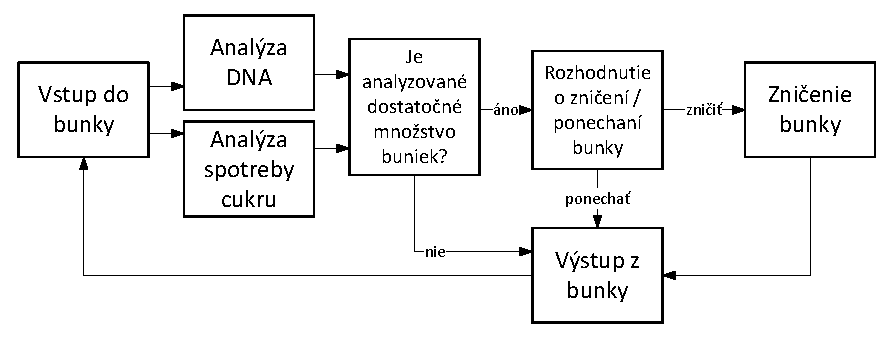
\includegraphics[scale=0.9]{spravanie.pdf}
\caption{Správanie nanobotov v organizme}
\end{figure}
%nebolo by lepsie tie vetviace krabicky spravit ako kosostvorce?
\section{Záver}

Problematika liečby rakoviny je veľmi obšírna a vyžaduje si inteligetné riešenie. Sú s tým spojené aj mnohé etické a filozofické otázky, taktiež aj bezpečnostné riziká. Čo ak sa niekomu podarí preprogramovať nanobotov, aby ničil zdravé bunky namiesto chorých? Budú ľudia ochotní takto splynúť s technológiou? Tieto a aj rôzne ďalšie otázky sú nezanedbateľné pri výskume tohto typu. Treba zhodnotiť, či potenciálny zisk vyváži riziko.

\listoffigures
\bibliography{zdroje}
\bibliographystyle{unsrt}
\end{document}

